%%%%%%%%%%%%%%%%
% This is an example CV created using altacv.cls (v1.3, 10 May 2020) written by
% LianTze Lim (liantze@gmail.com), based on the
% Cv created by BusinessInsider at http://www.businessinsider.my/a-sample-resume-for-marissa-mayer-2016-7/?r=US&IR=T
%
%% It may be distributed and/or modified under the
%% conditions of the LaTeX Project Public License, either version 1.3
%% of this license or (at your option) any later version.
%% The latest version of this license is in
%%    http://www.latex-project.org/lppl.txt
%% and version 1.3 or later is part of all distributions of LaTeX
%% version 2003/12/01 or later.
%%%%%%%%%%%%%%%%

%% If you are using \orcid or academicons
%% icons, make sure you have the academicons
%% option here, and compile with XeLaTeX
%% or LuaLaTeX.
% \documentclass[10pt,a4paper,academicons]{altacv}

%% Use the "normalphoto" option if you want a normal photo instead of cropped to a circle
% \documentclass[10pt,a4paper,normalphoto]{altacv}

\documentclass[10pt,a4paper,ragged2e,withhyper]{altacv}

%% AltaCV uses the fontawesome5 and academicon fonts
%% and packages.
%% See http://texdoc.net/pkg/fontawesome5 and http://texdoc.net/pkg/academicons for full list of symbols. You MUST compile with XeLaTeX or LuaLaTeX if you want to use academicons.

% Change the page layout if you need to
\geometry{left=0.9cm,right=0.9cm,top=0.9cm,bottom=0.9cm,columnsep=0.5cm}

% The paracol package lets you typeset columns of text in parallel
\usepackage{paracol}
\usepackage{multicol}
\usepackage{hyperref}
\usepackage{ragged2e}

%% timeline
\usepackage{tikz}
\usetikzlibrary{arrows.meta,
                chains,
                positioning}
% Change the font if you want to, depending on whether
% you're using pdflatex or xelatex/lualatex
\ifxetexorluatex
  % If using xelatex or lualatex:
  \setmainfont{Lato}
\else
  % If using pdflatex:
  \usepackage[default]{lato}
\fi

\makeatletter % <=======================================================
\renewcommand{\makecvheader}{%
  \begingroup
    \ifdef{\@photodiameter}{\begin{minipage}{\dimexpr\linewidth-\@photodiameter-3em}}{}% <=======
    \begin{minipage}{0.6\linewidth} % <=================================
      \raggedright\color{emphasis}%
      {\Huge\bfseries\MakeUppercase{\@name}\par}
      \medskip
      {\large\bfseries\color{accent}\@tagline\par}
    \end{minipage}
    \hspace{40pt}
    \begin{minipage}{0.35\linewidth} % <================================
      {\raggedleft\footnotesize\bfseries\@personalinfo\par}
    \end{minipage}
    \ifdef{\@photodiameter}{\end{minipage}\par}{}%
  \endgroup\medskip
}

\renewenvironment{fullwidth}{%
  \begin{adjustwidth}{}
  {\dimexpr-\marginparwidth-\marginparsep-2em\relax} % <================ added -2em
  }
  {\end{adjustwidth}}
\makeatother % <========================================================

% The lines below removes hyphenation
% \tolerance=1
% \emergencystretch=\maxdimen
\hyphenpenalty=10000
\hbadness=10000


% Change the colours if you want to

\definecolor{VividPurple}{HTML}{479099}
\definecolor{SlateGrey}{HTML}{2E2E2E}
\definecolor{LightGrey}{HTML}{444444}
% \colorlet{name}{black}
\colorlet{tagline}{VividPurple}
\colorlet{heading}{VividPurple}
\colorlet{headingrule}{VividPurple}
% \colorlet{subheading}{PastelRed}
\colorlet{accent}{VividPurple}
\colorlet{emphasis}{SlateGrey}
\colorlet{body}{LightGrey}

% Change some fonts, if necessary
% \renewcommand{\namefont}{\Huge\rmfamily\bfseries}
% \renewcommand{\personalinfofont}{\footnotesize}
% \renewcommand{\cvsectionfont}{\LARGE\rmfamily\bfseries}
% \renewcommand{\cvsubsectionfont}{\large\bfseries}

% Change the bullets for itemize and rating marker
% for \cvskill if you want to
\renewcommand{\itemmarker}{{\small\textbullet}}
\renewcommand{\ratingmarker}{\faCircle}
\setlength{\multicolsep}{6.0pt plus 2.0pt minus 1.5pt}% 50% of original values

%% sample.bib contains your publications
\addbibresource{sample.bib}

\begin{document}


\name{Gopal Ramesh Dahale}
\tagline{Undergraduate}

% Cropped to square from https://en.wikipedia.org/wiki/Marissa_Mayer#/media/File:Marissa_Mayer_May_2014_(cropped).jpg, CC-BY 2.0
%% You can add multiple photos on the left or right
% \photoR{2.5cm}{image.jpg}
% \photoL{2cm}{Yacht_High,Suitcase_High}
\personalinfo{%
% Not all of these are required!
% You can add your own with \printinfo{symbol}{detail}
\email{gopald@iitbhilai.ac.in}
\phone{+91 8425930185}
%  \mailaddress{Address, Street, 00000 County}
%   \location{Sunnyvale, CA}
%   \homepage{marissamayr.tumblr.com}
%   \twitter{@marissamayer}
\linkedin{gopal-ramesh-dahale-7a3087198}
\github{Gopal-Dahale} % I'm just making this up though.
%   \orcid{orcid.org/0000-0000-0000-0000} % Obviously making this up too. If you want to use this field (and also other academicons symbols), add "academicons" option to \documentclass{altacv}
%% You MUST add the academicons option to \documentclass, then compile with LuaLaTeX or XeLaTeX, if you want to use \orcid or other academicons commands.
% \orcid{0000-0000-0000-0000}
%% You can add your own arbtrary detail with
%% \printinfo{symbol}{detail}[optional hyperlink prefix]
% \printinfo{\faPaw}{Hey ho!}
%% Or you can declare your own field with
%% \NewInfoFiled{fieldname}{symbol}[optional hyperlink prefix] and use it:
% \NewInfoField{gitlab}{\faGitlab}[https://gitlab.com/]
% \gitlab{your_id}
}

\makecvheader

\emergencystretch=\maxdimen
% \begin{description}
%     \item[cxjdkfj] 
% \end{description}
%% Depending on your tastes, you may want to make fonts of itemize environments slightly smaller
\AtBeginEnvironment{itemize}{\small}

%% Set the left/right column width ratio to 6:4.
\columnratio{0.55}

% Start a 2-column paracol. Both the left and right columns will automatically
% break across pages if things get too long.
\begin{paracol}{2}

\cvsection{Education}
\begin{tikzpicture}[
    node distance = 1mm and 3mm, 
    start chain = A going below, 
    dot/.style = {circle, draw=white, very thick, fill=VividPurple, minimum size=3mm}, 
    box/.style = {rectangle, text width=100mm, inner xsep=4mm, inner ysep=1mm,                   font=\sffamily\small\linespread{0.84}\selectfont,on chain}]
\begin{scope}[every node/.append style={box}]
    \node { 
            \cvEd{BTech (Honours) in Electrical Engineering with specialization in Computer Science}{Indian Institute of Technology, Bhilai}{Aug 2018 -- Ongoing}{9.11/10.0}
            Coursework
            \setlength\multicolsep{0pt}
            \begin{multicols}{2}
                \begin{itemize}[noitemsep,topsep=0pt]
                    \item Graph Theory \& Applications
                    \item Operating Systems
                    \item Data Analytics \& Visualisation
                    \item Neural Networks \& Deep Learning (Coursera)
                \end{itemize}
            \end{multicols}
            \divider
    } ;
    \node { 
        \cvEd{High School}{Kendriya Vidyalaya, ONGC Panvel}{2017 -- 2018}{95.6 \%}
    } ;
\end{scope}
\draw[very thick, VividPurple, {Triangle[length=4pt)]}-{Circle[length=3pt]},
      shorten <=-1mm, shorten >=-1mm]           % <--- here is adjusted additional arrow's 
    (A-1.north west) -- (A-2.south west);
\foreach \i [ count=\j] in {1,2}
    \node[dot] at (A-\j.west) {};
\end{tikzpicture}

\cvsection{Projects}

\cvproject{Distribution \& Requirement of Medical Resources for Covid 19 \& Factors Affecting Hospitalization}{Sept 2020 - Nov 2020}{\href{https://github.com/Gopal-Dahale/Distribution-and-Requirement-of-Medical-Resources-for-Covid-19-and-Factors-Affecting-Hospitalization}{\underline{Link}}}{}

\begin{itemize}
  \item As a member of team of 5, analysed and \textbf{predicted the ICU admission of confirmed cases} using models like \textbf{Logistic Regression, ROC-AUC}.
  \item \textbf{Proposed a window model} to make the prediciton more clinically relevant and \textbf{achieved a R2-score of 0.8+} over test datasets.
  \item Extracted \& visualized weekly \textbf{hospitalization rates in USA} for various age-groups and medical conditions. 
  \item \textbf{\underline{Utilized:} Python, Pandas, NumPy, Plotly, Scikit-Learn.}
\end{itemize}
\divider

\cvproject{Playlist Creation}{Aug 2020 - Sept 2020}{\href{https://github.com/Gopal-Dahale/Automatic-Playlist-creation}{\underline{Link}}}{}

\begin{itemize}
\item Automated the task of playlist recommendation using a \textbf{scoring function based on Borda's method} for 3 different topics.
\item Extracted about \textbf{3000 videos data using Youtube Data API} using filters. Preprocessed, analysed and visualised the data \& Tabulated my results.
\item \textbf{\underline{Utilized:} Python, Matplotlib, Pandas, NumPy.}
\end{itemize}
\divider

\cvproject{Detecting Covid 19 with Chest X-rays}{July 2020- Aug 2020}{\href{https://github.com/Gopal-Dahale/Detecting-COVID-with-X-ray}{\underline{Link}}}{}
\begin{itemize}
    \item Classified Covid, viral \& normal cases using Resnet18 pretrained model. Transformed and augmented the data \& \textbf{achieved 0.95+ accuracy}.
    \item Deployed a \textbf{simple streamlit web app} to showcase the results.
    \item \textbf{\underline{Utilized:} Python, Pytorch, NumPy, Matplotlib,Streamlit,Flask.}
\end{itemize}
\divider

\cvproject{Covid 19 India Tracker}{May 2020 - June 2020}{\href{https://github.com/Gopal-Dahale/COVID19-India-Tracker}{\underline{Link}}}{}
\begin{itemize}
\item Developed an Android app using for \textbf{tracking Covid spread in Indian states \& districts}. Illustrated the data using India map. 
\item Preprocessed the data obtained from \href{https://github.com/covid19india/api}{\underline{covid19india/api}}.
\item \textbf{\underline{Utilized:} Kotlin, Javascript.}
\end{itemize}
\divider

\cvproject{Load Flow Analysis}{Feb 2020 - April 2020}{\href{https://github.com/Gopal-Dahale/Load-flow-analysis}{\underline{Link}}}{}
\begin{itemize}
\item Solved the \textbf{Load-Flow problem using Guass-Seidel} iterative method.
\item \textbf{\underline{Utilized:} C++.}
\end{itemize}





% \divider

% \cvevent{Product Engineer}{Google}{23 June 1999 -- 2001}{Palo Alto, CA}

% \begin{itemize}
% \item Joined the company as employe \#20 and female employee \#1
% \item Developed targeted advertisement in order to use user's search queries and show them related ads
% \end{itemize}

% \cvsection{A Day of My Life}

% Adapted from @Jake's answer from http://tex.stackexchange.com/a/82729/226
% \wheelchart{outer radius}{inner radius}{
% comma-separated list of value/text width/color/detail}
% Some ad-hoc tweaking to adjust the labels so that they don't overlap
% \hspace*{-1em}  %% quick hack to move the wheelchart a bit left
% \wheelchart{1.5cm}{0.5cm}{%
%   10/13em/accent!30/Sleeping \& dreaming about work,
%   25/9em/accent!60/Public resolving issues with Yahoo!\ investors,
%   5/11em/accent!10/\footnotesize\\[1ex]New York \& San Francisco Ballet Jawbone board member,
%   20/11em/accent!40/Spending time with family,
%   5/8em/accent!20/\footnotesize Business development for Yahoo!\ after the Verizon acquisition,
%   30/9em/accent/Showing Yahoo!\ \mbox{employees} that their work has meaning,
%   5/8em/accent!20/Baking cupcakes
% }

% use ONLY \newpage if you want to force a page break for
% ONLY the currentc column
% \newpage

% \cvsection{Publications}

% \nocite{*}

% \printbibliography[heading=pubtype,title={\printinfo{\faBook}{Books}},type=book]

% \divider

% \printbibliography[heading=pubtype,title={\printinfo{\faFile*[regular]}{Journal Articles}}, type=article]

% \divider

% \printbibliography[heading=pubtype,title={\printinfo{\faUsers}{Conference Proceedings}},type=inproceedings]

%% Switch to the right column. This will now automatically move to the second
%% page if the content is too long.
\switchcolumn

% \cvsection{Life Philosophy}
% \begin{quote}
% ``If you don't have any shadows, you're not standing in the light.''
% \end{quote}

\cvsection{Experience}

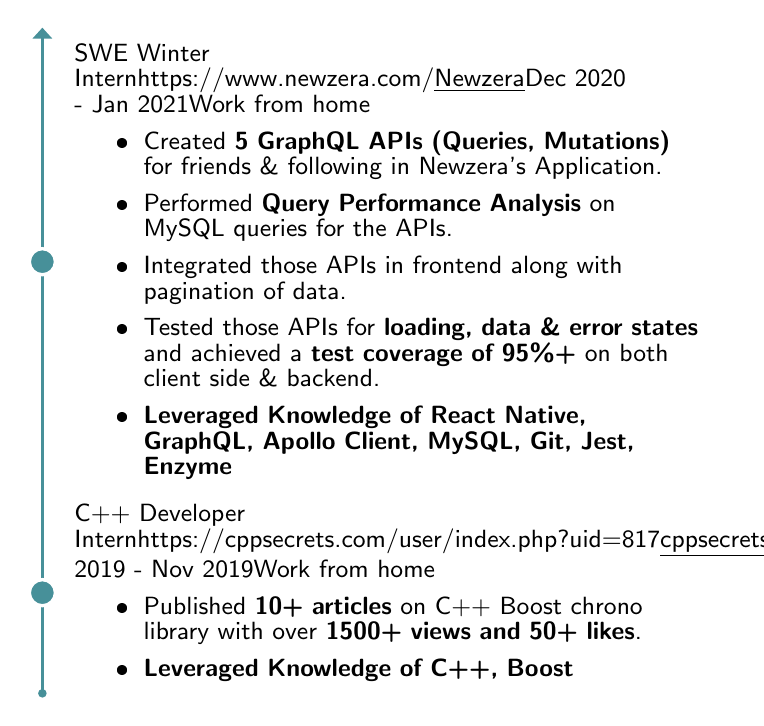
\begin{tikzpicture}[
    node distance = 1mm and 3mm, 
    start chain = A going below, 
    dot/.style = {circle, draw=white, very thick, fill=VividPurple, minimum size=3mm}, 
    box/.style = {rectangle, text width=80mm, inner xsep=4mm, inner ysep=1mm,                   font=\sffamily\small\linespread{0.84}\selectfont,on chain}]
\begin{scope}[every node/.append style={box}]
    \node {
        \cvevent{SWE Winter Intern}{\href{https://www.newzera.com/}{\underline{Newzera}}}{Dec 2020 - Jan 2021}{Work from home}
        \begin{itemize}
        \item Created \textbf{5 GraphQL APIs (Queries, Mutations)} for friends \& following in Newzera's Application.
        \item Performed \textbf{Query Performance Analysis} on MySQL queries for the APIs.
        \item Integrated those APIs in frontend along with pagination of data. 
        \item Tested those APIs for \textbf{loading, data \& error states} and achieved a \textbf{test coverage of 95\%+} on both client side \& backend.
        \item \textbf{Leveraged Knowledge of React Native, GraphQL, Apollo Client, MySQL, Git, Jest, Enzyme}
        \end{itemize}
        \divider
    } ;
    \node {
        \cvevent{C++ Developer Intern}{\href{https://cppsecrets.com/user/index.php?uid=817}{\underline{cppsecrets.com}}}{Aug 2019 - Nov 2019}{Work from home}
        \begin{itemize}
        \item Published \textbf{10+ articles} on C++ Boost chrono library with over \textbf{1500+ views and 50+ likes}.
        \item \textbf{Leveraged Knowledge of C++, Boost}
        \end{itemize}
    } ;
\end{scope}
\draw[very thick, VividPurple , {Triangle[length=4pt)]}-{Circle[length=3pt]},
      shorten <=-1mm, shorten >=-1mm]           % <--- here is adjusted additional arrow's 
    (A-1.north west) -- (A-2.south west);
\foreach \i [ count=\j] in {1,2}
    \node[dot] at (A-\j.west) {};
\end{tikzpicture}

\cvsection{Strengths}
Proficient:
\cvtag{C/C++}\cvtag{HTML/CSS/Javascript}\cvtag{Python}

\divider

Familiar: 
\cvtag{Kotlin}\cvtag{React Native}\cvtag{GraphQL}\cvtag{MySQL}\cvtag{Jest/Enzyme}\cvtag{Pytorch}\cvtag{Scikit-learn}\cvtag{Firebase}\cvtag{Flask}\cvtag{Streamlit}\cvtag{\LaTeX}

\cvsection{Achievements}

\cvmyachievement{Completed an online course Data Analysis with Python organised by \href{https://www.jovian.ai/?utm_source=webapp}{\underline{Jovian.ai}} }{Aug 2020 - Sept 2020}{\href{https://jovian.ai/dahalegopal27}{\underline{Credential}}}

\cvmyachievement{Participated in 30 days of Kotlin campaign organised by Google.}{May 2020 - June 2020}{\href{https://drive.google.com/file/d/1FGPYe8gs3-1bRX9CPSY-AxNC3qklIU8p/view}{\underline{Credential}}}

\cvmyachievement{Completed Responsive Web Design Developer Certification from \href{https://www.freecodecamp.org/}{\underline{freeCodeCamp}}}{Jan 2020 - March 2020}{\href{https://www.freecodecamp.org/certification/fccdcf64cea-ae73-4db1-8f4b-2f30b4fa70bdg/responsive-web-design}{\underline{freeCodeCamp}}}

\cvmyachievement{Verified Skills \& Badges on HackerRank}{Jan 2019 - Sept 2020}{\href{https://www.hackerrank.com/dahalegopal27}{\underline{Credentials}}}

\cvmyachievement{Earned Qwiklabs Essential Badges from Google Cloud Training}{Aug 2019 - Sept 2019}{\href{https://google.qwiklabs.com/public_profiles/80cfcdb6-e310-48fe-b59b-662f3924c6fd}{\underline{Badges}}}



% \divider\smallskip

% \cvtag{UX}
% \cvtag{Mobile Devices \& Applications}
% \cvtag{Product Management \& Marketing}

% \cvsection{Languages}

% \cvskill{English}{5}
% % \divider

% \cvskill{Spanish}{4}
% % \divider

% \cvskill{German}{3}


% \newpage

% \cvsection{Referees}

% % \cvref{name}{email}{mailing address}
% \cvref{Prof.\ Alpha Beta}{Institute}{a.beta@university.edu}
% {Address Line 1\\Address line 2}

% \divider

% \cvref{Prof.\ Gamma Delta}{Institute}{g.delta@university.edu}
% {Address Line 1\\Address line 2}

\end{paracol}
\end{document}